%   MSc Business Analytics Dissertation
%
%   Title:     Literature Review
%   Author: Conor Reid
%
%   Chapter 3: Literature Review
%
\chapter{Literature Review}\label{C.LitReview}
\section{Introduction}\label{S.intro3}
{This literature review first presents some of the ways that corporate success can be quantified. We look at how it is defined by \cite{moldovan2015learning}, as well as by others whose approaches may benefit this study. Also included here is a discussion of various fronts on which companies act, such as their corporate social responsibility commitments, with a view to including these aspects in this analysis as independent explanatory features. This is followed by an analysis of existing literature on the relationship between corporate governance and company performance, again including the work of \cite{moldovan2015learning} as well as other relevant studies. This review finishes with an exploration of literature regarding causation and the statistical techniques used to infer causation. There is also discussion on the issues that arise in attempting to do so, and how they can be addressed. }
\section{Company Performance - Measures and Influencers}\label{comPerform}
\subsection{Introduction}
{Among the key aspects of this study is the quantifying of corporate success, in a way that accurately   represents good and bad corporate performance. There are many aspects to this. One of the easiest ways to measure corporate economic success is to use financial ratios, many of which have been developed that attempted to assign numerical performance ratings to companies taking into account varying amounts of accounting indictors. \cite {eidleman1995z} outlines the patterns that ratios tend to follow. He states that these ratios are mostly created by academic researchers, who constantly derive new ways of combining individual metrics together to facilitate meaningful comparison between companies. First, researchers find a sample of companies that meet some predetermined criterion of failure, as well as another sample of comparable firms (size, industry etc) that differ only in financial health. A number of ratios are developed and tested against this dataset so analyse which return values that are consistently and significantly different for each group. Those which do so are kept, the rest are discarded. Weights are assigned to each ratio to reach an aggregate equation. New firms are scored, and real-world performance recorded to measure how useful the new ratios are in practice. \\\\
This study primarily considers corporate governance features as predictors of corporate economic success. This follows the lead of \cite{moldovan2015learning} who do the same. Having said this, an aim of this study is to expand the range of predictors considered, and to this end we discuss alternative sources of company data that can be incorporated into the model. Perhaps the inclusion of more varied and diverse independent covariates, such as the companies social responsibility commitments and  impact on the environment can enhance understanding in this domain. These areas are discussed in this chapter.    }
\subsection{Financial Ratios}\label{FinancialRatios}
{Some financial ratios or more useful than others, since they vary significantly in complexity and in what particular aspects of a company they consider. This section includes a discussion of some of the most commonly used ratios, with comments on how best they can be used and in what context they are most powerful. \\\\
One of the indicators of corporate performance used by \cite{moldovan2015learning} is Tobin's Q score. This measure was devised by \cite{tobin1969general} who postulated that the combined market value of a given company should be equal to their replacement costs. When a companies replacement cost is equal to its market value, it is said to be in an ideal state. Any deviation either way, a ratio above or below 1, warrants investment or the selling of assets respectively. \cite{moldovan2015learning} argue that the Q score allows the estimation of intangible assets, and is thus a worthy inclusion as a dependant measure of corporate success. Intangible assets drive market value up, rising the Q score.  \\\\
The use of this measure is well established elsewhere in the literature also, for example by \cite{chung1994simple}, 
\cite{bhagat2008corporate} and \cite{bolton2011unified}. \cite{chung1994simple} state that Tobin's Q plays an important part in financial interactions, and is employed to explain diverse corporate phenomena during the decision making process. \cite{bolton2011unified} used Tobin's Q to propose a model for dynamic investment and risk management and found that investment is best driven by the Q score as well as to the marginal value of liquidity. \\\\
The formal definition of Tobin's Q is presented by \cite{chung1994simple}, along side a much more simplified and conservative approximation of the authors making. This less complex definition is given below as; \\
\begin {equation}\label{TobinQ}
(Approximate) \quad q  = \small {\frac{MVE + PS + DEBT}{TA}}
\end{equation}
In the equation above, $MVE$ represents the product of a companies share price and count of common outstanding stock shares. $PS$ represents the liquidating value of the companies preferred stock. $DEBT$ represents the companies short-term liabilities minus its assets, also short-term. Finally, $TA$ represents the book value of the total assets of the company. In layman terms, assets that cannot be easily quantified can not always be entered in a companies books, but do always contribute to the share price of that company. Thus, a firm with lots of this type of asset will have a high Q score.\\\\ 
There is debate as to the practically of the Q score. Intuitively, the Q score places a very high importance on one specific aspect of a business. For example, before WhatApp was acquired by Facebook it had very little concrete physical assets. Rather, it had a platform with approximately 400million users, and a very high Q score. After purchase, the Q score would have dropped significantly since the amount Facebook paid would become the concrete asset recorded in their books. This is not to say that the Q score is a bad success indicator, but rather it may not fully represent the real value of a company at a given time.\\\\    \cite{chung1994simple} state in their research that the Q score is often neglected in real-world situations. One of the reasons they give for this is the complexity of the necessary calculations, and a potential unfamiliarity with its operational intricacies. Another reason is the unavailability of relevant data, particularly of sufficiently high accuracy and temporal availability. To counteract this, they worked to create and test an accurate approximation of Tobin's Q that utilises only basic financial information, show in equation \ref{TobinQ}.  They conclude that their approximation is close enough to the more formal definition to be used where more exhaustive calculations are not possible. \\\\
%\cite {dybvig2010tobin} criticise Tobin's Q more strongly, stating that it is fundamentally malformed as a measure of corporate performance. They highlight long-serving managers as risk adverse, and who "...can {\it enjoy the quiet life} and underinvest". A logical implication of this is that firms invest less and operate well below their profit-generating capacity and thus reduces their net-present value. However, such is Tobin's Q formulated, underinvestment by a firm increases its Q score. They go on to explain the scores ambiguity, COME BACK TO. \\\\
Another measure of corporate success used by \cite{moldovan2015learning} is the Altman Z score, which is often used as a probabilistic measure of whether a company will go into bankruptcy within the next two years. It can also be used more generally as a financial distress measure and to predict corporate defaults. The authors point out that there is much advocacy in the literature for using this measure, and this study was unable to find any that strongly reject its usefulness. The Altman Z score is given as;
\begin {equation}\label{AltmanZScore}
\begin{aligned}
Z \ Score \quad = \quad & 1.2\bigg(\frac{Working \ Capital}{Total \ Assets}\bigg) \ + \\\\
		& 1.4\bigg({\frac{Retained \ Earnings}{Total \ Assets}}\bigg) \ + \\\\
		& 3.3\bigg({\frac{Earnings \ before \ Interest \ and \ Tax}{Total \ Assets}}\bigg) \ + \\\\
		& 0.6\bigg({\frac{Market \ Value \ of \ Equity}{Total \ Liabilities}}\bigg) \ + \\\\
		& 1.0\bigg({\frac{Sales}{Total \ Assets}}\bigg)
\end{aligned}
\end{equation}\\
Among those that support this scores use is \cite {eidleman1995z}, who discusses its use in practice. He begins by highlighting Altman's own tests using the Z score which involved predicting 72\% of bankruptcies two years prior to the event, although the sample size or companies involved are not mentioned. Eidleman argues that the Z score is tried and tested, and;
\begin {quote}
It has been demonstrated to be quite reliable in a variety of contexts and countries. 

\hspace{2cm}---  \cite {eidleman1995z}
\end{quote}
Eidleman also outlines circumstances that warrant corrections and alterations to equation \ref{AltmanZScore}, in order to generalise it beyond its originally intended means. He argues that before being able to use the Z score, one must ensure the company in question is comparable to those involved in Altman's original study. Altman considered manufacturing and small firms in his original analysis, thus corrections must be made before scoring companies in different industries. Eidelman points to two specific circumstances here. \\\\
The first considers privately held companies, whose stocks are no publicly traded meaning term four of equation \ref{AltmanZScore} cannot be calculated. To correct for this, the Z score can be re-estimated using book values of equity. In other words, details from balance sheets published by private firms voluntarily can be used rather than details gleamed from the stock market. Certainly a work-around here is to consider solely publicly traded companies. A consequence of this is that such an analysis would only include companies that are bound by the the corporate governance code in their jurisdiction, which would need to be taken into account in studies such as this one.\\\\ Eidleman's second consideration is for non-manufacturing firms. The fifth term of equation \ref{AltmanZScore}, according to Eidleman, varies significantly by industry. He argues that merchandise firms for example, are significantly less capital intense and thus are much more likely to enjoy higher asset turnover and consequently Z-Scores. Z scores then would be likely to under-predict bankruptcy in these cases. In order to correct for this, a recommendation comes from Altman to eliminate the fifth term and adjust the weights. 
\clearpage
The adjusted equation \ref{AltmanZScoreAjusted} is shown below;
\begin {equation}\label{AltmanZScoreAjusted}
\begin{aligned}
Z \ Score \quad =  \quad & 6.56\bigg(\frac{Working \ Capital}{Total \ Assets}\bigg) \ + \\\\
		& 3.26\bigg({\frac{Retained \ Earnings}{Total \ Assets}}\bigg) \ + \\\\
		& 6.72\bigg({\frac{Earnings \ before \ Interest \ and \ Tax}{Total \ Assets}}\bigg) \ + \\\\
		& 1.05\bigg({\frac{Market \ Value \ of \ Equity}{Total \ Liabilities}}\bigg) \ \\\\ 
\end{aligned}
\end{equation}\\
Overall, the Altman Z score seems a highly appropriate indicator of corporate financial strength and thus success, and one that should be considered in this study. Consideration will need to be had for the type of industry included in this analysis, that will inform the exact calculation of the Z score itself. }
\subsection{Environmental Considerations}\label{EnvironmentalConsiderations}
{As mentioned previously, there is likely much room for improvement in the range of predictors of success considered in this analysis. One potentially useful area to consider is the environmental performance of the company, studied by \cite{schaltegger2002link}. The authors primary focus is on environmental management, specifically as a vehicle for corporate success. It is assumed here that environmental management and performance relate to the controlling of costs relating perhaps to the mining of natural resources. This may also refer to fines, penalties or taxes that are incurred due to harmful emissions, which must be carefully managed within a company to mitigate against. \\\\
The authors present two conflicting viewpoints in this space. The first states that improved environmental performance predominantly causes an increase in operating costs, due to investment and so on which in turn negatively effects the profitability of the company. The second viewpoint states the opposite; improving a firms environmental performance in fact induces cost savings, which drives increases in profitability. Interestingly, the authors present opinions that environmental investment often both negatively increases costs and positively increases income. Having said this, they argue that such a direct link is not present in practice, and that instead it is the identification and management of the relationship that is more important. The conflicting viewpoints are visualised in figure \ref{ch3_successAndEnviornment}. 
\begin{figure}[h] 
\centering
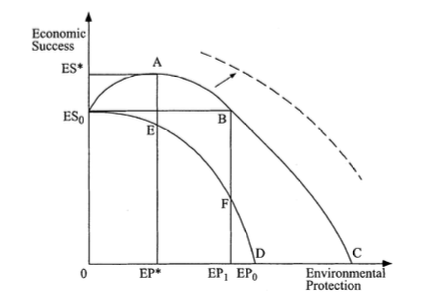
\includegraphics[scale = 0.7]{images/ch3_successAndEnviornment.png}
\caption{Correlation between corporate environmental protection spending and economic success.}
\label{ch3_successAndEnviornment}
\end{figure}\\
$ES_0$ on the vertical axis represents the current level of economic success, described by the authors a certain shareholder value. According the the pessimistic view of environmental spending, this value decreases as spending in environmental protection increases (through points E and F, to D where non profit can be made). That is, spending in this space reduces profit making ability to eventual zero. The more optimistic view is represented by the path from $ES_0$ through points A and B to point C (again where no profit is possible). This represents the ideology that some economic gain can be achieved, at least to some degree before tailing off, by being environmentally conscious. Of course, even in this situation there is an optimal investment level, after which profit making ability decreases. \\\\
The authors draw point to two important ideas, derived from figure \ref{ch3_successAndEnviornment}. First, they argue that environmental performance can vary at a given level of economic success. It is both possible to be equally successful by being either environmental friendly or harmful. This indicates that investment in this space does not necessarily mean poor economic performance. Secondly, the reverse; that economic success can vary for a given level of environmental protection. That is, being environmentally conscious is no guarantee of economic benefit. The authors reiterate that the correlation between economic and environmental performance depends on not just company externalities but internal variables which are influenced by management. It is firm management, who moderate this relationship, that must be optimised in order to gain economically. The authors put this forward as an group of explanatory covariates not considered in the literature to this point. \\\\
It is natural then to ask how environmental management can be quantified in data for analysis. \cite{schaltegger2002link} suggest two cases for deriving data. The first relates to the firms ability to utilise to the full the economic benefits of environmental protection measures. This may materialise in R\&D spending, or other marketing positioning that communicates their efforts and establishes the company as industry leaders. They are seen as quality leaders, with their environmental management policies a significant driver of this. The second case relates to how this reputation is achieved in practice, by realising the optimal environmental performance for maximum economic success. This can take the form of identifying and implementing optimise production processes for example, facilitated by the identification of opportunities and "eco-efficiency potentials". \\\\
\cite{wahba2008does} also performs research in this area, studying whether the market values corporate environmental responsibility, specifically in an Egyptian context. Similarly to \cite{schaltegger2002link}, the author acknowledges divided and inconclusive literature on this topic, stating an aim to present empirical evidence on how engagement with environmental responsibility can positively influence corporate market value. This analysis looks at a sample of 156 firms across 19 industries, using the market value of a firm as the dependant variable (interestingly, quantified by Tobin's Q score mentioned previously). Important to note is the authors use of ISO 14000/14001 certification as a proxy for environmental performance. This is recognised by the authors as non-ideal, however this may still have some utility in future research to address the difficulty in quantifying performance in this area. \\\\
An interesting and important consideration is made by \cite{wahba2008does}. She states that companies with greater economic success have a greater ability to invest in environmental endeavours, leading to a theory that the two may be jointly determined. This theory is tested before regression analysis run. To do this, the author uses the specification test of \cite{hausman1978specification} to test for endogeneity. Endogeneity occurs in econometrics when an explanatory variable correlates with the error term, rather than some other feature. \cite{wahba2008does} states that the result of this analysis is that endogeneity is not occurring, but points to an important consideration that the current study may need to take into account. One of the common causes of this is a causal loop between an independent and a dependant variable, and can obviously lead to wildly inaccurate results. \\\\
 \cite{wahba2008does} state that the overall finding of this research is that the market does in fact reward firms for their environmental efforts, by positively influencing that firms Tobin's Q score, but do point to similar issues raised by \cite{schaltegger2002link}. Namely, that a companies decision to reduce their impact on the environment comes with significant cost and that if this is not managed correctly, the economic benefits evaporate.     \\\\
There is clear support in the literature for the presence of a relationship between corporate economic success and environmental performance. \cite{schaltegger2002link} suggest it is the firm management of environmental considerations that influences success, and put this forward as an explanatory variable not yet considered in literature. This theory is supported by \cite{wahba2008does}, who find a strong relationship in this space but with a caveat that management plays a significant role in realising benefits. It remains to be seen exactly how this can be realised in data analysis, and what family of covariates could be incorporated into the model.  }
\subsection{Corporate Social Responsibility}
{Corporate social responsibility, or CSR, is defined by the European Commission as "the responsibility of enterprises for their impacts on society". This is similar to being conscious of environmental impact, but is more generalised to include compliance with established ethical standards and national and international norms. Central to CSR is the creation of shared value between themselves, their stakeholders and larger society as well as mitigating possible adverse events with those groups. It is natural to consider elements of CSR then, when discussing predictors of firm success. \\\\
\cite{orlitzky2003corporate} perform meta-analysis in the link between corporate social and financial performance. They begin by stating;
\begin{quote}
Most theorising on the relationship between corporate social / environmental performance (CSP) and corporate financial performance (CFP) assumes that the current evidence is too fractured or too variable to draw any generalisable conclusions.

\hspace{2cm}--- \cite{orlitzky2003corporate}
\end{quote}
Their research aims to show this claim is unfounded, and that it is indeed possible to derive insight in this space by providing a more rigorous methodology for drawing such conclusions. They argue that researchers have attempted to find causal relationships between CSP and CSR, but have failed in part due to a failure to see vital differences between theory and operational applications. They also state that an aim of their research is to aggregate knowledge in the area, and highlight important findings they believe to be overlooked. This type of meta-analysis have been proven to provide value by considering a number of disparate and conflicting results holistically, by reaching an aggregate conclusion.\\\\
They present a number of hypotheses about the influence of CSP. They first state that CSP and CFP are positively related, regardless of industry and the context of the given study relating the two. They base this on a number of studies, stating that CSP is a vital form of "good management theory" that boasts competitive advantage by addressing stakeholder concerns quickly and fairly.  Secondly, they hypothesise on the temporal nature of this relationship, and further that there is a bidirectional causality between CSR and CFP. That is, there is a circular and virtuous casual relationship that governs performance in each area. This is supported by the idea that prior success in CFP facilitates positive engagement in CSP, due to increased responsibility and freedom at the managerial level. This conclusion mirrors that seen in section \ref{EnvironmentalConsiderations}, where it was theorised that increased economic success drives better environmental performance.\\\\
The third hypothesis put forward by \cite{orlitzky2003corporate} involves the underlying logic behind the correlation between CSP and CFP. The first is that CSP boasts managerial competencies and organisational efficiency, by enabling shared knowledge of the firm's market as well as social and political environments. Secondly they suggest that CSP is a driving factor behind the firm's reputation, and thus elicits significant goodwill from stakeholders. \\\\
The fourth and final hypothesis put forward involves the methodology used by previous studies to draw conclusions from. The authors here suggest that the variance in results seen across studies can be explained by sampling or measurement error, for example. \\\\
In order to support these claims, \cite{orlitzky2003corporate} perform a meta-analysis involving 52 studies across both CSP and CFP, resulting in a total sample size of 33,878 observations on which they perform their analysis. This analysis involves a statistical aggregation technique to be applied, which calculates the cumulative correlations across studies, correcting for variable elements of those studies to reach one "true score correlation ($\rho$)". Using this technique, the authors were able to explain 24\% of the cross-study variance in relation to the observed r value, which they suggest is significant. That is, by controlling for sampling and measurement errors across multiple studies, they could reduce the variation in results by 25\%. They suggest that this, strengthened with other analysis, supports their collection of hypotheses.\\\\
The authors compare their results with others who performed similar research. Key to this comparison is a discussion regarding the linkage between CSP and CFP. That state that other researchers have traditionally been concerned with the "Halo effect". That is, that correlation found (that CSP influences CFP) are due to the experimental procedure or are spuriously perceived. The authors here dismiss this, stating that the only logical halo link would be in the reverse direction. That is, that a company who are high financially successful may be scored highly in CSP regardless of factual information in that regard. They go further, and state that even this hypothetical (but more logical) argument is debunked by their meta-analysis which shows a strong directional (or temporal) link between CSP and CFP. \\\\
As as with environmental performance, there is clear evidence that corporate social performance (or perhaps more commonly, responsibility) is a worthy addition to this study. Along side governance features and the aforementioned environmental performance features, there is evidence that CSP can enhance predictive power and understanding in this domain.    }
\section{Corporate Governance and Company Performance}
\subsection{Introduction}
{In this chapter, we explore research directly in the same domain as the current study. That is, other works that look at the relationship between corporate governance and company performance. This includes the work of \cite{moldovan2015learning}, whose research forms the basis for the current study. An analysis is made of their methodology and conclusions, as well as a deeper analysis of what areas can be improved upon.}
\subsection{Existing research}
{\cite{moldovan2015learning} made an attempt to find relationships between how a company governs, and its economic success using data mining. They derived a dataset from the Bloomberg financial system, containing 50 independent corporate governance features on areas such as board room structure and the  companies yearly tax and interest liabilities. They considered three stock indexes; S\&P 500 (a collection of 500 american companies), STOXX Europe 600 and STOXX Eastern Europe 300. They complimented this with two dependant, target variables measuring corporate success. They are Tobin's Q and the Altman Z Score, the details both of which are included in section \ref{comPerform}. Using the aforementioned governance variables, they learned statistical models to predict {\it good} and {\it bad} company performance.\\\\
Interestingly, \cite{moldovan2015learning} decided to discretise Tobin's Q into two classes, one for a {\it good} score and the other for a {\it bad} score split by the median score. They carry out similar preprocessing on the Altman Z score, creating three classes and allocating observations to each based on performance before using a classification algorithm for learning purposes. While the authors cite this methodology in previous literature, it may prove interesting to allow these variables to remain as real-valued, and perform regression analysis. We believe this alternative methodology may yield positive results. \\\\
The formulation of the Altman Z score use by \cite{moldovan2015learning} is also an area for potential concern. As discussed in section \ref{FinancialRatios}, Altman presents an alternative formulation for non-manufacturing companies that prevents under estimation of bankruptcy likelihood. It remains to be seen what kind of companies are included in this analysis, although should a significant number fall outside of the manufacturing industry then perhaps the alternative formulation should be used.   \\\\
Using a number of different algorithms, \cite{moldovan2015learning} were able to highly accurately predict corporate outcomes using governance features. Interestingly, results for the American and European datasets were very similar across algorithms which good performance in each case. Results from the Eastern European dataset were less promises, attributed to missing data on the governance side. Promisingly, no algorithm was shown to be significantly better than any other across datasets. \\\\
As mentioned previously, the authors here were able to present some simple rules based on their models for corporate governance best practice. For example, they conclude that there is a positive correlation between women on the board of directors in American companies, thresholding on 20\% presence for the benefits to activate. An independent lead director in the same dataset was shown to incur a higher risk of bankruptcy as measured by the Altman Z score. In Europe, the authors came to a similar conclusion, stating that the presence of an independent lead director or former CEO on the board of directors resulted in poorer Tobin Q scores. Interestingly and contrary to the case in America, the presence of women on the board was negatively linked to performance. Finally, in Eastern Europe \cite{moldovan2015learning} found that a smaller director age range was positively related with performance. Altman Z scores improve significantly with an independent chairman, or female CEO. 
}
\section{Inferring Causation}
\subsection{Introduction}
{It is stated ad nauseum in scientific and popular literature that "Correlation does not imply causation" or similar. In statistical analysis, it is tempting to infer causal relationships between features where only correlation has been proven and indeed a significant amount of literature seems to do exactly this. For example, the study of \cite{moldovan2015learning} on which the current study is based, makes string claims as to the relationships between corporate governance and company success. In reality, the authors perform insufficient analysis to support such claims, instead finding correlations worthy of further investigation. \\\\
Interestingly, there is a significant body of research that argues that it is impossible to prove causation. It is said that if all variables that could possibly be causal are considered, causation can be reliably inferred. Of course in practice this is almost never the case, and so issues around $<>$ require advanced techniques to address and potentially overcome.     \\\\
One of the major issues with applying causal research in this domain is the study design. Many studies, particularly in the medical field, are able to take advantage of robust experimental design standards that facilitate a deep and accurate exploration of results. They are able to control for unobserved covariates using randomised trials, and generally have a large degree of control over the statistical parameters of the study. The goal here is often to maintain a treatment and control group, and estimate that treatments effect on outcomes.  \\\\
Outside of such a highly controlled environment, causal inference becomes more difficult where we begin to deal with observational studies. The work of \cite{moldovan2015learning} is such a study, where they authors derived historical data that was generated outside of their control and tried to uncover relationships within. \cite{esarey2015causal} identifies an interesting problem with this type of work. Often, the act of choosing to be treated has a significant effect on outcomes. He gives the example of education; those who choose to complete higher education may be those who stand to gain from it the most, and so it is difficult to estimate educations effect on income. Similarly in the study of \cite{moldovan2015learning}, it is difficult to assess the benefit of various elements of corporate governance on firm performance due to the self-selecting nature of those who perform well in the former. There is an implicit temporal element to this discussion, and indeed \cite{pearl1995theory} state that often temporal precedence is normally assumed to be essential to defining a causal relationship. They argue that this alone cannot distinguish causation however, and point to research stating that unless one knows all potentially causal covariates it is impossible to make this step at all. \\\\
This is a highly complex space, and one that certainly calls for advanced techniques that can mitigate the issues outlined above. The remainder of this section is dedicated to some of these techniques, with discussion of their technicalities and practical applications.  }
\subsection{Matching}\label{matching}
{One approach to bridging the gap between experimental and non-experimental studies is matching, outlined by \cite{stuart2010matching} who considers studies that use observational data that can be divided into treated and non-treated cases. Matching is then used to study the effects of this treatment on some outcome, in a very similar way to standard experimental trials in the medical field for example. He describes first how one of the biggest benefits of randomised experimental studies is that the treated and un-treated groups are guaranteed to be randomly different from one another, on both observed and unobserved covariates (or features that may influence the outcome). That is, such experiments are able to control for factors that have not been explicitly designed for in the experiment. Statistical matching aims to imitate this for observational studies, by balancing the distribution of potentially useful features in the treated and control groups. This is achieved by identifying observations that differ only in treated status, facilitating the analysis of the causal effect of that treatment. In effect this ignores un-observed features, and aims to reduce bias in the distribution of observed features as much as possible. The concept of {\it strong ignorability} is heavy relied upon here, which is to say that it is assumed that all feature that may influence the outcome are being considered. \\\\
\cite {stuart2010matching} identifies matching as a potentially useful mechanism in supervised learning, where the outcome is known and the goal is to estimate its effect. Thus, matching is considered in this study where the treatment can be quantified as fluctuations in various explanatory corporate governance variables (among others) which in turn influence the a firms outcome. \\\\
\cite {stuart2010matching} sets out four key stages in the matching process. They are;
\begin {enumerate}
\item{Defining the measure of {\it closeness}.}
\item{Choosing an appropriate matching method.}
\item{Quality assessment of matched samples, returning to step 1 depending on results.}
\item{Treatment analysis, given the results of Step 3.}
\end{enumerate}
A measure of closeness quantifiably determines whether an observation is a good match for another. This is a crucial aspect to matching, and can be subdivided into two parts. The first involves pruning the dataset features for those to include, taking into consideration {\it strong ignorability}. \cite{stuart2010matching} points out that poor results are expected from using small sets of features, particularly those that pertain solely to a narrow view of that observation (for example, demographic details of individuals). He states that there is little disadvantage in including features that are not actually associated with outcome, albeit a slight increase in variance is expected. Conversely, neglecting a feature that is associated with outcome is very costly, and so it is recommended to include as many features as is practical as a precaution. It is also recommended to do so without relying on observed outcomes, and instead make decisions based on domain knowledge. \\\\
%put in something here about type of variables not to include
The second aspect to closeness is the measure of distance itself, or the similarity between two observations in the data. There are many ways to do this, that vary in the exactness of the match required. \cite{stuart2010matching} argues that exact matching is ideal, but very often unattainable especially with high dimensional data. Requiring a very high degree of exactness leads to observations remaining unmatched which then fall out of consideration, a phenomenon that in turn can lead to more bias than if the matching measure required less exactness. A way to address this is to categorise continuous features, a practice used in calculating the Mahalanobis distance for example which works well with low dimensionality, but poorly with highly non-uniformly distributed features.
\\\\ 
The next stage in the matching process is the choose of matching method, which uses the closeness distance to create the matches themselves. The motivation behind using one method over another lies in the number of observations that remain after matching has taken place, and the relative weights that different individuals receive. One such method is nearest neighbour matching (NNM), which is stated as the most common, most understandable and easiest to implement methods available by \cite{stuart2010matching}. In essence, this method couples a treated and un-treated observation, minimising the distance between the two. Controls can be put in place to dictate the exactness of each match, potentially discarding treated cases if a suitable match is not found. This helps to prevent bad matches, but leads to difficulties in interpreting results. What results from NNM is a data set of similar dimension to the amount of treated cases, which arguably reduces the power of the data. \cite{stuart2010matching} states in response to this that model precision is effected most by the smaller group size in any dataset, and so balancing observations down to this smaller group size should not in fact dramatically reduce it power. 
\\\\
The third stage of the matching process is a quality assessment of the matched samples, which is the most important step according to \cite{stuart2010matching}. The aim here is to rate how balanced the matches set is, where balance refers to the similarity of feature distributions, and the independence of features and treatment status. Poor results here calls for alternative distance measures and matching methods, and so iteration is often required to find the optimal methodology. \cite{stuart2010matching} proposes numerical diagnostics to achieve this step. This involves the inspection of the difference in means of each feature, divided by the standard deviation which gives the {\it standard bias}. This is performed for each feature, as well as their two-way interactions and squares. The author discards other common tests here such as hypothesis tests, due to contextual issues and how balance is interpreted by those tests. 
 \\\\ 
The fourth and final step of the matching process as outlined by \cite{stuart2010matching} is outcome analysis. It should be noted that matching is not actually a tool used for inferring causation, but rather presents a new dataset that is treated as if sourced through randomised methods.  
\\\\
\cite{king2014balance} also characterise the trade-off between matched sample sizes and the balance between classes into the matched subset, identified above by \cite{stuart2010matching}. While \cite{stuart2010matching} argued that any negative effects of sample reduction were offset by the increased balance between groups, \cite{king2014balance} argues the opposite. They claim that practitioners often do see sample reduction as an issue, citing manual tweaking that research cary out in an effort to optimise sample size as well as balance, or their tendency to settle for suboptimal solutions. \cite{king2014balance} argue that optimising only one of these parameters is not a viable solution nor a necessary one, but that current solutions available for optimising both require significant manual intervention which is time consuming and usually suboptimal. In response to this, they propose a new approach that they claim address a number of issues. \\\\
The so called {\it matching frontier} is a methodology that the authors claim fully characterises the trade-off between dataset imbalance and matched sample size, allowing researchers to visually inspect where the optimal solution lies for a given dataset. Each location along the frontier is denoted by the resultant matched sample. Moving along this frontier (i.e. varying sample size), the frontier returns a data subset such that no other subset of the same size has more optimal class balance characteristics. That is, the returned matched dataset is optimally balanced for its size. The implications of this for researchers are obvious. Using this method, one has much finer control over the matching process than is apparent in the work of  \cite{stuart2010matching}. The latter provides a framework that involves significant manual iteration, which is shown to be suboptimal and unnecessary by \cite{king2014balance}. }
\subsection{Minimal-Model Semantics}
{\cite{pearl1995theory} present a highly influential theory of causation, and guidelines on how to make the step from strong correlation towards inferring casual relationships. This is certainly one of the more influential studies in this space, and approaches the problem of causation slightly differently to matching laid out in section \ref{matching}. The authors here propose what they refer to as {\it a minimal-model semantics of causation}, which they claim debunk the myth that casual influences cannot be distinguished from illegitimate covariation. They argue this is possible through inductive reasoning.\\\\
They begin by stating generalities of proving causation, and of causal systems. Firstly, they state that intelligent systems that aim to learn about their environment and act on that knowledge cannot rely solely on preprogrammed causal knowledge (derived from human knowledge and experience). Rather, it must be able to transform observable phenomenon into cause and effect relationships. They argue further that when causal relationships are stated in ordinary conversation, they reflect probabilities of event occurring rather than absolutes. Thus, probability theory should be sufficient to identify such relationships. it is clear that the authors place a large degree of faith in ordinary people, going as far as to say of peoples ability to perceive causal relationships {\it "..we must find a computational model that emulates this perception"}. It remains to be seen whether this is the most fruitful avenue of exploration.\\\\
Key to the model proposed by \cite{pearl1995theory} is the notion of a directed acyclic graph (DAG). The authors theorise that fundamentally, all processes in nature are controlled by casual mechanisms that govern how observable and unobservable variables interact. In general, they state that;
\begin{quote}
A casual model of a set of variables U is a directed acyclic graph (DAG), in which each node corresponds to a distinct element of U. 

\hspace{2cm}---  \cite {pearl1995theory}
\end{quote}
Variables are representable as nodes, with edges representing casual influences between those variables. Using this model, it becomes clear how the influence of parent variables on child variables can be found. One of the issues that has been raised in this chapter previously is that of the influence of unobservable factors, which are impossible to eliminate in practice. The authors here model these as probabilistic disturbances to the DAG, that perturbs the relationships within. This is certainly a novel approach, and presents a theoretical framework for dealing with inevitable externalities.\\\\
\cite {pearl1995theory} on go to discuss the question of model structure and choice. Logically, since the model $U$ is not bounded by any predetermined constraint (i.e. inputted casual knowledge or otherwise) there in an infinite amount of models that could be fitted to a given distribution. Each would create different causal relationships with a different set of probabilistic disturbances. The authors call on inductive reasoning here, arguing that any model can be removed if there is a more simple alternative that is as consistent with the data. Models not removed are referred to as {\it minimal models}, and are used to reach the authors definition of inferred causation. 
\begin{quote}
A variable X is said to have a casual influence on a variable Y if a strictly directed path from X to Y exists in every minimal model consistent with the data. 

\hspace{2cm}---  \cite {pearl1995theory}
\end{quote}

--------------------\\
Much more to review in this paper including:
\begin{enumerate}
\item{Stability - Computational Practicality}
\item{Latent Structures}
\item{Non-temporal causation}
\item{Attached algorithm to make this happen}
\end{enumerate}
\section{Research Gap}
{}


}